\documentclass{article}
\usepackage{amsmath}
\usepackage{hyperref}
\usepackage{amsfonts}
\usepackage{bookmark}
\usepackage{float} 
\usepackage{graphicx}
\usepackage{makeidx}
\usepackage[letterpaper, total={7.5in, 10in}]{geometry}


\makeindex
\begin{document}
\title{Test 1 \\
    Semester 2}
\author{Elias Xu}
\date{\today}
\maketitle

\section{Introduction}

Here are Multi Notes to prepare for the first test

\section{Double Integrals}

Double integrals are integrals that represent the volumes under a surface, rather than \textbf{Definite Integrals}, which compute the area under a curve.

\subsection{Definite Integrals Recap}

\begin{figure}[H]
    \centering
    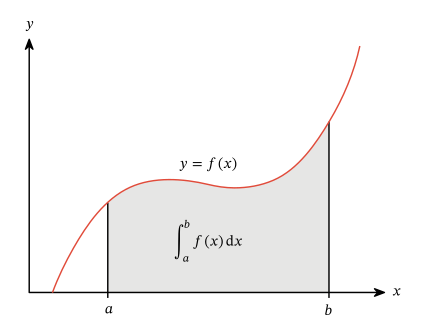
\includegraphics[width=0.2\textwidth]{images/DefiniteIntegralExample.png}
    \caption{Example of a definite Integral}
\end{figure}


Integrals are limits of a Riemann sum, which can be represented by the following equation:
$$\int_{a}^{b} f(x)\delta x = f(x_1)\Delta x_1 + f(x_2) \Delta x_2 + ... = \lim_{n \to \infty} \sum_{i = 1}^{n} f(x_i) \Delta x_i \text{ ,where } \max \Delta x_i \to 0$$

\subsection{Applying Definite Integrals to double integrals}

\begin{figure}[H]
    \centering
    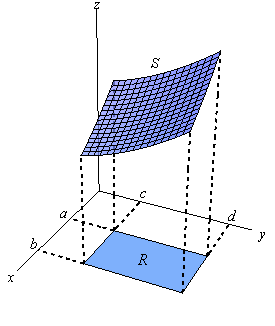
\includegraphics[width=0.2\textwidth]{images/DoubleIntegralsExample.png}
    \caption{Example of a double Integral}
\end{figure}

Given that we have to find the area underneath the curve of a function $z = f(x,y)$, we will need to find \textbf{volume}, not area.\\
We're going to define the rectangle area by:
$$R = \lbrace (x, y) | a \le x \le b , c \le y \le d \rbrace = [a,b] \times [c, d] \text{ (Cartesian Sum)}$$ \\
And thus we can define a solid $S$ using the equation:
$$S = \lbrace  (x, y, z) | (x, y) \in \mathbb{R}, 0 \le z \le f(x, y) \rbrace$$ \\
If one is to use equal subintervals to calculate, then you can use a double Riemann sum, with the area of a rectangle equal to $\Delta x \times \Delta y \times f(x,y)$.
You can represent that sum, with
$$\lim_{m, n \to \infty}\sum_{j=1}^{m} \sum_{i=1}^{n} f(x_i^*, y_i^*)\Delta A$$ \\
(\textbf{NOTE} the *'s mean that the values are at a specific point) Where m and n represent the number if subintervals. \\
Double Riemann sums give volume, which when "limited" simplifies to
$$\iint_{R} f(x, y) \delta A = \iint_{[a, b] \times [c, d]} f(x,y) \delta A$$

\subsection{Notes}


\begin{enumerate}
    \item If $f(x, y) \ge 0 \text{ and } f(x, y) \in \mathbb{R}$ then $\iint_{R} f(x, yA) = $ is the volume of the solid bounded by x, y, and the surface
    \item $\delta A = \delta x \delta y \text{ or } \delta y \delta x$. Order will impact evaluation but not result.
    \item If $f(x, y)$ is continious in  $R$, then the double integral exists. (\textbf{NOTE}: You can get away with some discontinuity, such as with steps and the like, but not with stuff like infinite behavior)
\end{enumerate}





\end{document}